\documentclass[10pt,preprint,numbers]{sigplanconf}

\usepackage{times}
\usepackage{datetime}
\usepackage{url}
\usepackage{hyperref}
\usepackage{todonotes}

%\conferenceinfo{}{}
\copyrightyear{2018} 

\title{Intra-Process Piping: Accelerating Process Ensembles with
Software Fault Isolation}
% No date in title area.
\date{}

% Paper number and no. of pages as author
\authorinfo{Paper \textbf{\#XX}}{NN pages}

%\author{Yiwen Li \and Sam Weber \and Justin Cappos \and Brendan Dolan-Gavitt}

\begin{document}

\maketitle

\begin{abstract}

A proposed benefit of software fault isolation (SFI)~\cite{Wahbe:1993}
is that it can improve the performance of applications made up of
multiple isolated components communicating via remote procedure calls
(RPC). There is now a mature and widely used SFI implementation for the
x86-64 architecture (Google's Native Client, or NaCl), designed for
hosting untrusted code inside a web browser environment. In this paper,
we address the question of whether SFI can provide a performance
improvement over process-based isolation for modern Linux systems,
without compromising reliability or security. We design and implement an
SFI system based on Native Client with the specific goal of accelerating
ensembles of process that communicate via UNIX pipes, such as those
commonly found in shell scripts, and consider what architectural changes
in the last twenty years (most notably the widespread adoption of 64-bit
address spaces) make an SFI-based approach practical. In our
experiments, we demonstrate that our \emph{Intra-Process Pipe (IPP)}
system gives speedups of up to XXX\% on a collection of shell scripts
found in a standard Ubuntu 16.04 distribution, and speedups of up to
XXX\% on pipelines found in the authors' own shell histories,
making it attractive for speeding up UNIX shell scripts and day-to-day
usage.

\end{abstract}

\section{Introduction}
\label{sec:intro}

Many common data manipulation and analysis tasks can be carried out in
the UNIX environment by composing pipelines of built-in utilities. This
technique of building up complex functionality out of simple utilities,
often referred to as the \emph{UNIX philosophy}~\cite{unixphilosophy},
remains popular in industry and academia, despite decades of
criticism~\cite{unixhaters}. Without wading into this debate, we will
simply observe that this style of programming typically leads to
pipelines composed of a large number of processes communicating with one
another. Because context switching is expensive on many
architectures~\cite{contextswitch}, including the widely-used 64-bit x86
architecture, pipelines can often be slower than a monolithic program
with the same functionality.

One solution to the high cost of context switching is to stop relying on
hardware to enforce isolation between processes, and instead construct
software so that it cannot interfere with other running processes, even
if those processes happen to share the same address space. This
approach, known as \emph{Software Fault Isolation
(SFI)}~\cite{Wahbe:1993}, isolates programs by placing them into a
logical \emph{fault domain} (a portion of the larger address space) and
then ensuring that the cannot jump to or reference memory outside of
their domain. More recently, Google's Native Client~\cite{Yee:2009}
provided a practical, performant (around 7\% slowdown on
x86-64~\cite{Sehr:2010}) implementation of SFI intended to allow users
to run untrusted binary applications inside the Google Chrome web
browser.

\todo[inline]{Brendan: We need to do some more thinking about why SFI for standard
UNIX processes makes more sense now than it did 24 years ago.}

Despite the availability of a practical SFI implementation, the promise
of accelerating inter-process communication has not yet been achieved.
This appears to be due to two factors: first, aside from memory
isolation, achieving resource and performance isolation inside a single
address space remains challenging. Second, when SFI was initially
proposed, the majority of architectures had only 32 bits' worth of
address space available, which meant that the number of programs that
could be placed in the same address space was severely limited. This has
changed with the widespread adoption of 64-bit architectures; on a
standard Linux system, 128TB of address space is now available to each
user space process, making it practical to house many processes in a
single address space. We further reflect and elaborate on these
architectural shifts and how they make SFI an attractive choice for
accelerating UNIX pipelines on today's architectures in
Section~\ref{sec:discussion}.

In this paper, we present the design and implementation of
\emph{Intra-Process Pipes (IPP)}, a technique for accelerating shell
script pipelines by moving separate processes into the same address
space. Aside from the requirement that each program and its libraries be
compiled using the Native Client compiler, no changes are necessary to
the operating system or programs. A thin runtime library wraps the
OS interface to provide resource isolation and implements a fast
intraprocess communication mechanism. This runtime also smooths over the
differences between processes and threads, for example by ensuring that
signals sent to the process are delivered to the appropriate thread. The
details of the IPP design and implementation can be found in Sections
\ref{sec:design} and \ref{sec:implementation}, respectively.

\todo[inline]{Brendan: We should briefly summarize what experiments we did, what
workloads show improvement.}

We conclude that moving process pipelines is an idea whose time has
come: on a variety of real-world workloads, IPP can provide significant
speedups without sacrificing the reliability and safety benefits of
hardware isolation.

\section{Related Work}
\label{sec:relwork}

\subsection{Software Fault Isolation}

The core of our system is based on \emph{software fault isolation}, an
idea first proposed by Wahbe et al., who developed the idea of placing
constraints on binary code in order to isolate each component into a
\emph{logical fault domain}, with isolation enforced by software rather
than hardware protection. Although this line of research initially
focused on RISC architectures with fixed-length instructions, other
researchers~\cite{Small:1997,Erlingsson:2000} extended this work to the
variable-length x86 instruction set by adding runtime checks to ensure
that control flow transfers go to a predefined set of targets. McCamant
et and Morrisett~\cite{McCamant:2006} introduced key techniques (such as
forced alignment of instructions with \texttt{nop} padding) that allow
reliable disassembly of x86 binaries, making them amenable to
verification. Around the same time, Ford and Cox~\cite{Ford:2008}
demonstrated a different approach to sandboxing native code. Their
system, VX32, used dynamic binary translation combined with the segment
registers available on 32-bit x86 to isolate code with minimal slowdown
(and, in some cases, a performance \emph{improvement} due to improved
code cache locality).

This somewhat crowded field was joined by Google's Native Client
(NaCl)~\cite{Yee:2009}. Native Client combines ideas from multiple
previous systems, such as the use of reliable disassembly and
segmentation-based memory isolation, and adds a trusted runtime in the
same process to provide a secure monitor for external calls; a
springboard/trampoline system provides secure control flow transfer to
and from the trusted runtime. Because the 64-bit x86 architecture
dropped support for hardware memory segmentation (and other
architectures, such as ARM, never supported it in the first place), the
Native Client team later developed several new
techniques~\cite{Sehr:2010} that allow NaCl to be efficiently
implemented on x86-64 and ARM. Native Client is included in the Google
Chrome web browser in order to allow untrusted web sites to run native
code safely in the browser (in contrast to earlier systems such as
Microsoft's ActiveX, where vulnerabilities in components would lead to
the compromise of entire browser). This means that the NaCl codebase is
more mature and ``battle-tested'' than most research systems, which
makes it an attractive base on which to implement our own system.

\subsection{Language-Based Isolation}

Earlier isolation based on high-level languages: SPIN (Modula-3)~\cite{Bershad:1995}

Singularity OS, specifically \cite{Hunt:2007} and \cite{Hunt:2007a} and \cite{Aiken:2006}

\subsection{Improving IPC/RPC Performance}

Lots and lots of stuff here. SFI paper cites a lot but there has been
tons of interest due to its relevance to microkernels.

\section{Design}
\label{sec:design}


\section{Implementation}
\label{sec:implementation}

\section{Experiments}
\label{sec:experiments}

To demonstrate that our \emph{Intra-Process Pipe (IPP)} system is a practical solution to 
providing speedups without sacrificing the reliability and safety benefits of hardware isolation, 
we conducted experiments on both microbenchmarks and real-world workloads. 

\todo[inline]{Yiwen: Besides the performance results we are showing here, should we also add experiments 
demonstrating the reliability and safety of our system? Maybe we can show examples such as an attacker 
tried to access memory address in cage B from inside of Cage A, but failed. Or maybe we can talk about this 
in the Discussion section.}

\subsection{Microbenchmarks}
\label{experiments.microbenchmarks}

The purpose of our microbenchmark experiments was to demonstrate that by introducing intra-process pipe, 
communication between two processes through our user-space pipe would be faster than using the traditional 
pipe, which will invoke system calls into the operating system kernel that incur context switches. 

Our microbenchmark experiments were conducted in the following way. 
Two programs were communicating through one pipe. One program was sending data over through the write side of the pipe. 
The other program was receiving data through the read side of the pipe. 
The experiments were conducted in both native Linux, and in our IPP system. 
We compared the performance in both environments, as the size of the data block being sent changed. 
Results are shown in Figure \ref{fig:microbenchmarks}. 
IPP has performance improvement up to 50\% against native Linux.  

\begin{figure}
\centering
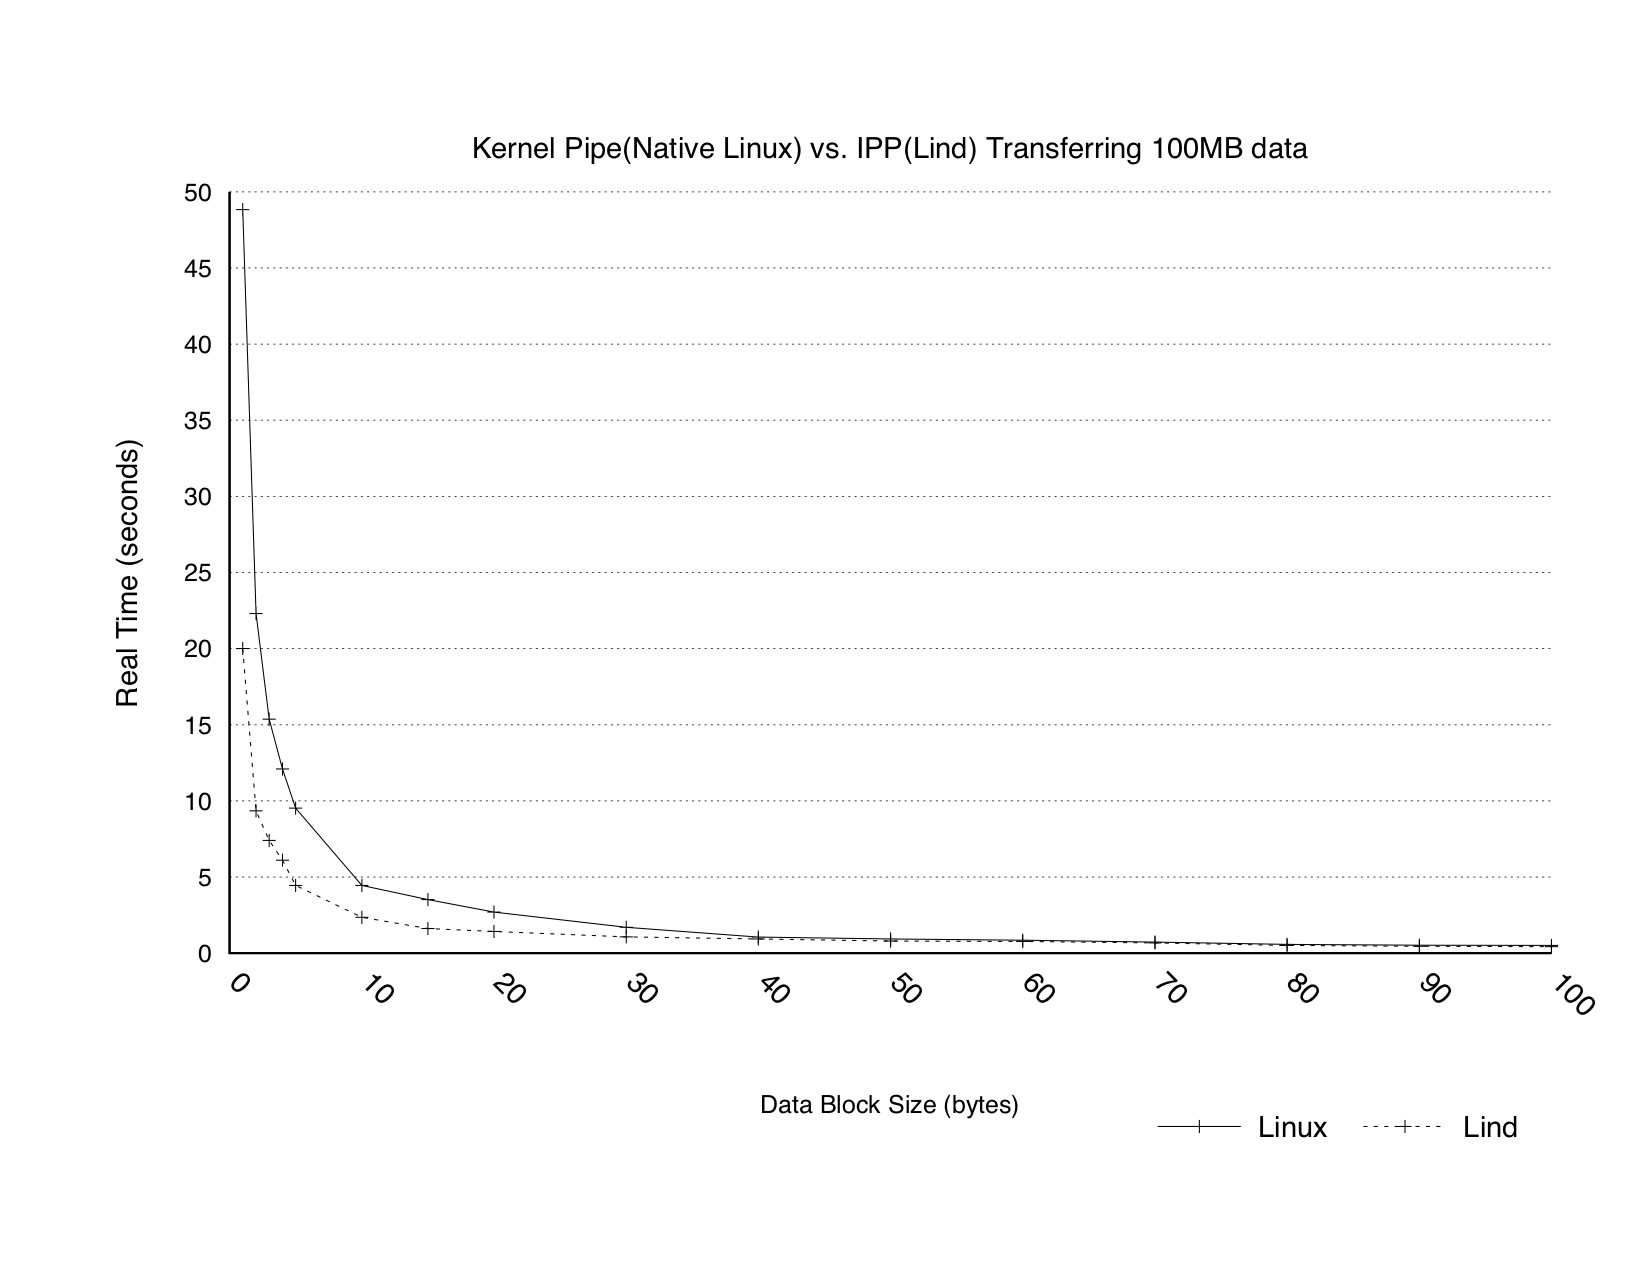
\includegraphics[width=1.0\columnwidth]{diagram/microbenchmarks.png}
\caption{\small Microbenchmarks: Linux vs. IPP.}
\label{fig:microbenchmarks}
\end{figure}

\subsection{Real-World Workloads}
\label{experiments.real-world_workloads}

Next, we conducted experiments on a collection of bash pipeline commands. 
The reasons that we chose bash pipeline commands to run the experiments are: 
first, bash pipeline commands are being widely used by programmers, developers, and researchers 
on Linux and Mac OS. Second, in many cases, bash pipeline commands are easier to use and could be more effective 
than complex programs or tools such as Hadoop. 
We collected and tested a set of real-world bash pipeline commands. Through our experiments, our goal is to demonstrate that 
our \emph{Intra-Process Pipe (IPP)} system provides an attractive solution to speeding up widely used bash pipeline commands 
on real-world workloads. 

We now show the nine real-world bash pipeline commands we tested. Each test was ran under both native Linux and our IPP system. 

\noindent
\textbf{Experiment 1.}

\noindent
\textbf{Setup.}
The following bash pipeline command was from one of the authors' bash history. 
\texttt{grep IOADDR * | sed 's/.*: //' | tr ' ' '\textbackslash n' | sort | uniq -c | sort -n} 
We ran this command on a 1.2GB dataset. 

\noindent
\textbf{Results.}
Results are shown in Figure \ref{fig:results01}. 
We see speedup up to 18\% in our IPP system. 

\begin{figure}
\centering
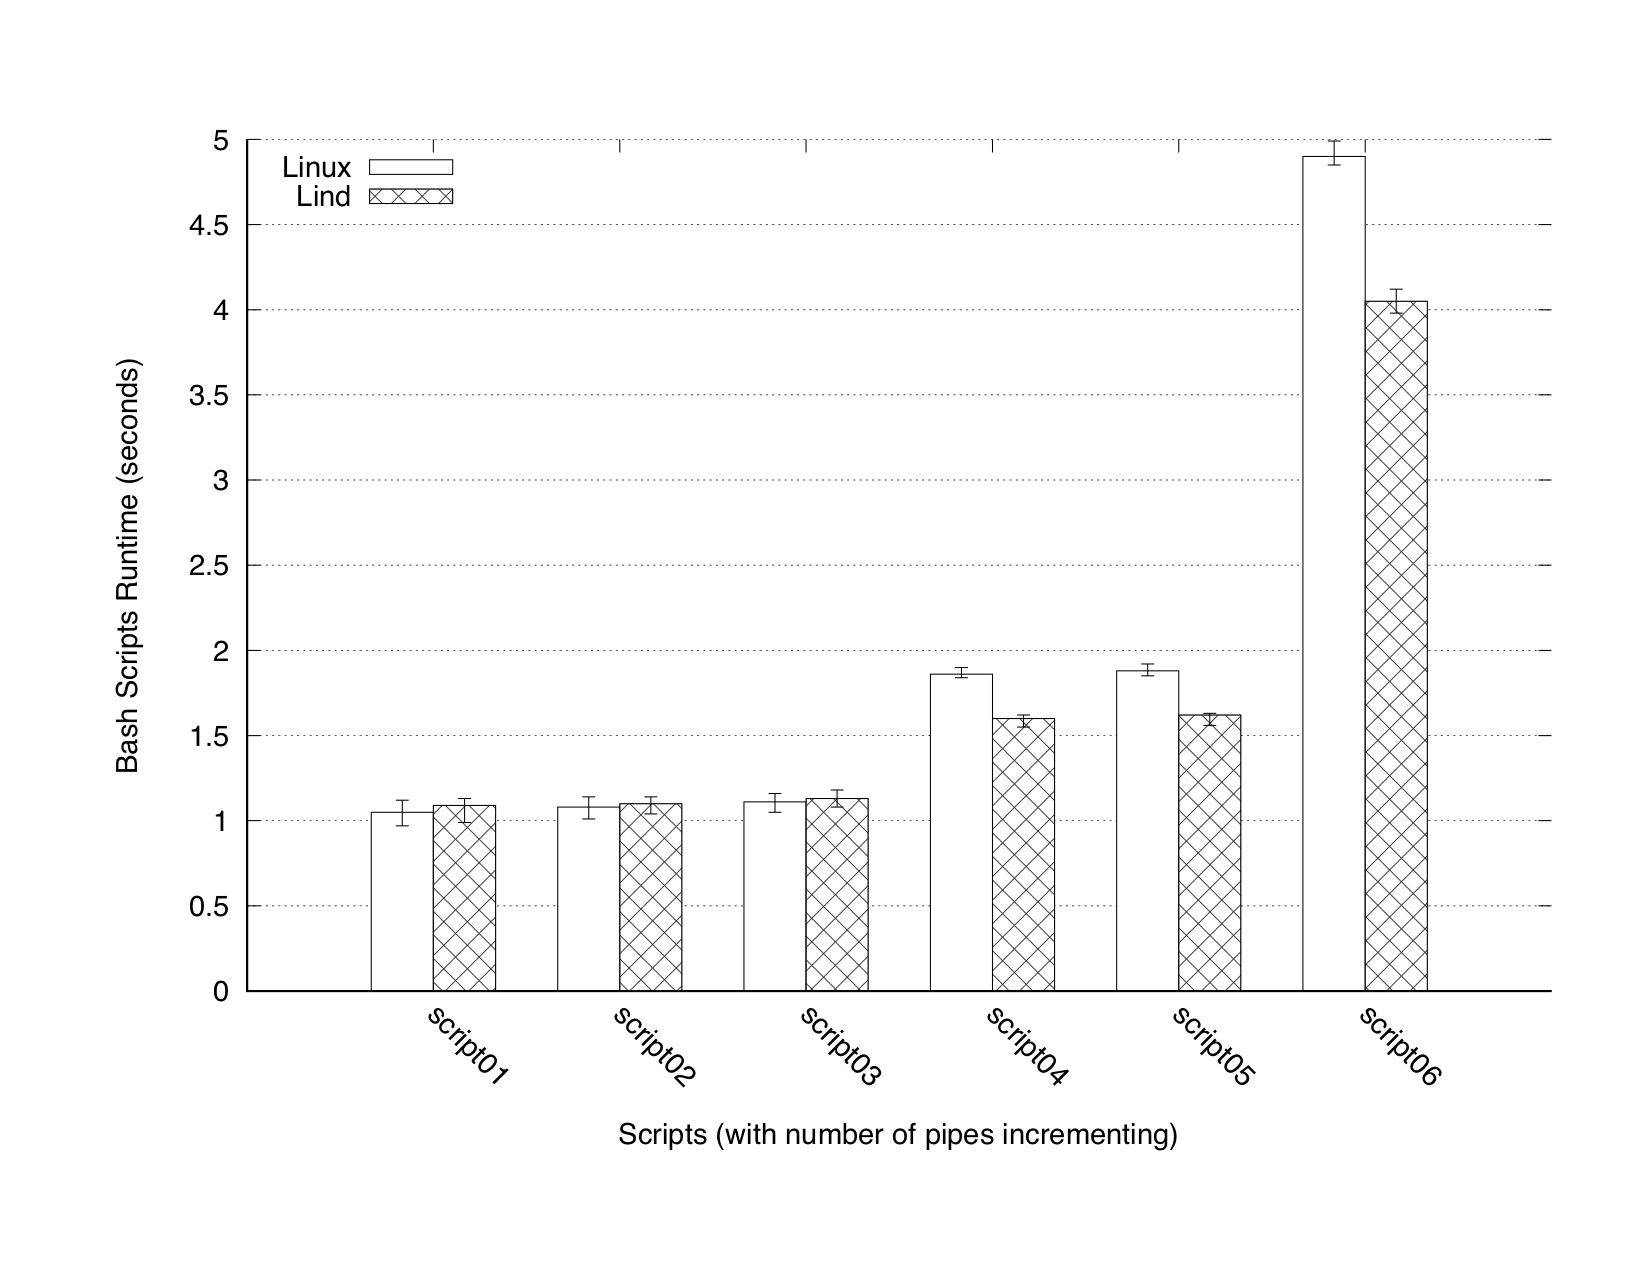
\includegraphics[width=1.0\columnwidth]{diagram/results01.png}
\caption{\small Real-World Workload 1.}
\label{fig:results01}
\end{figure}

\noindent
\textbf{Experiment 2.}

\noindent
\textbf{Setup.}

\texttt{cat ./dataset/pgn/*.pgn | grep "Result" | sort | uniq -c > ./results/results.txt} 


\noindent
\textbf{Results.}
Results are shown in Figure \ref{fig:results02}. 
We see speedup up to 20\% in our IPP system. 

\begin{figure}
\centering
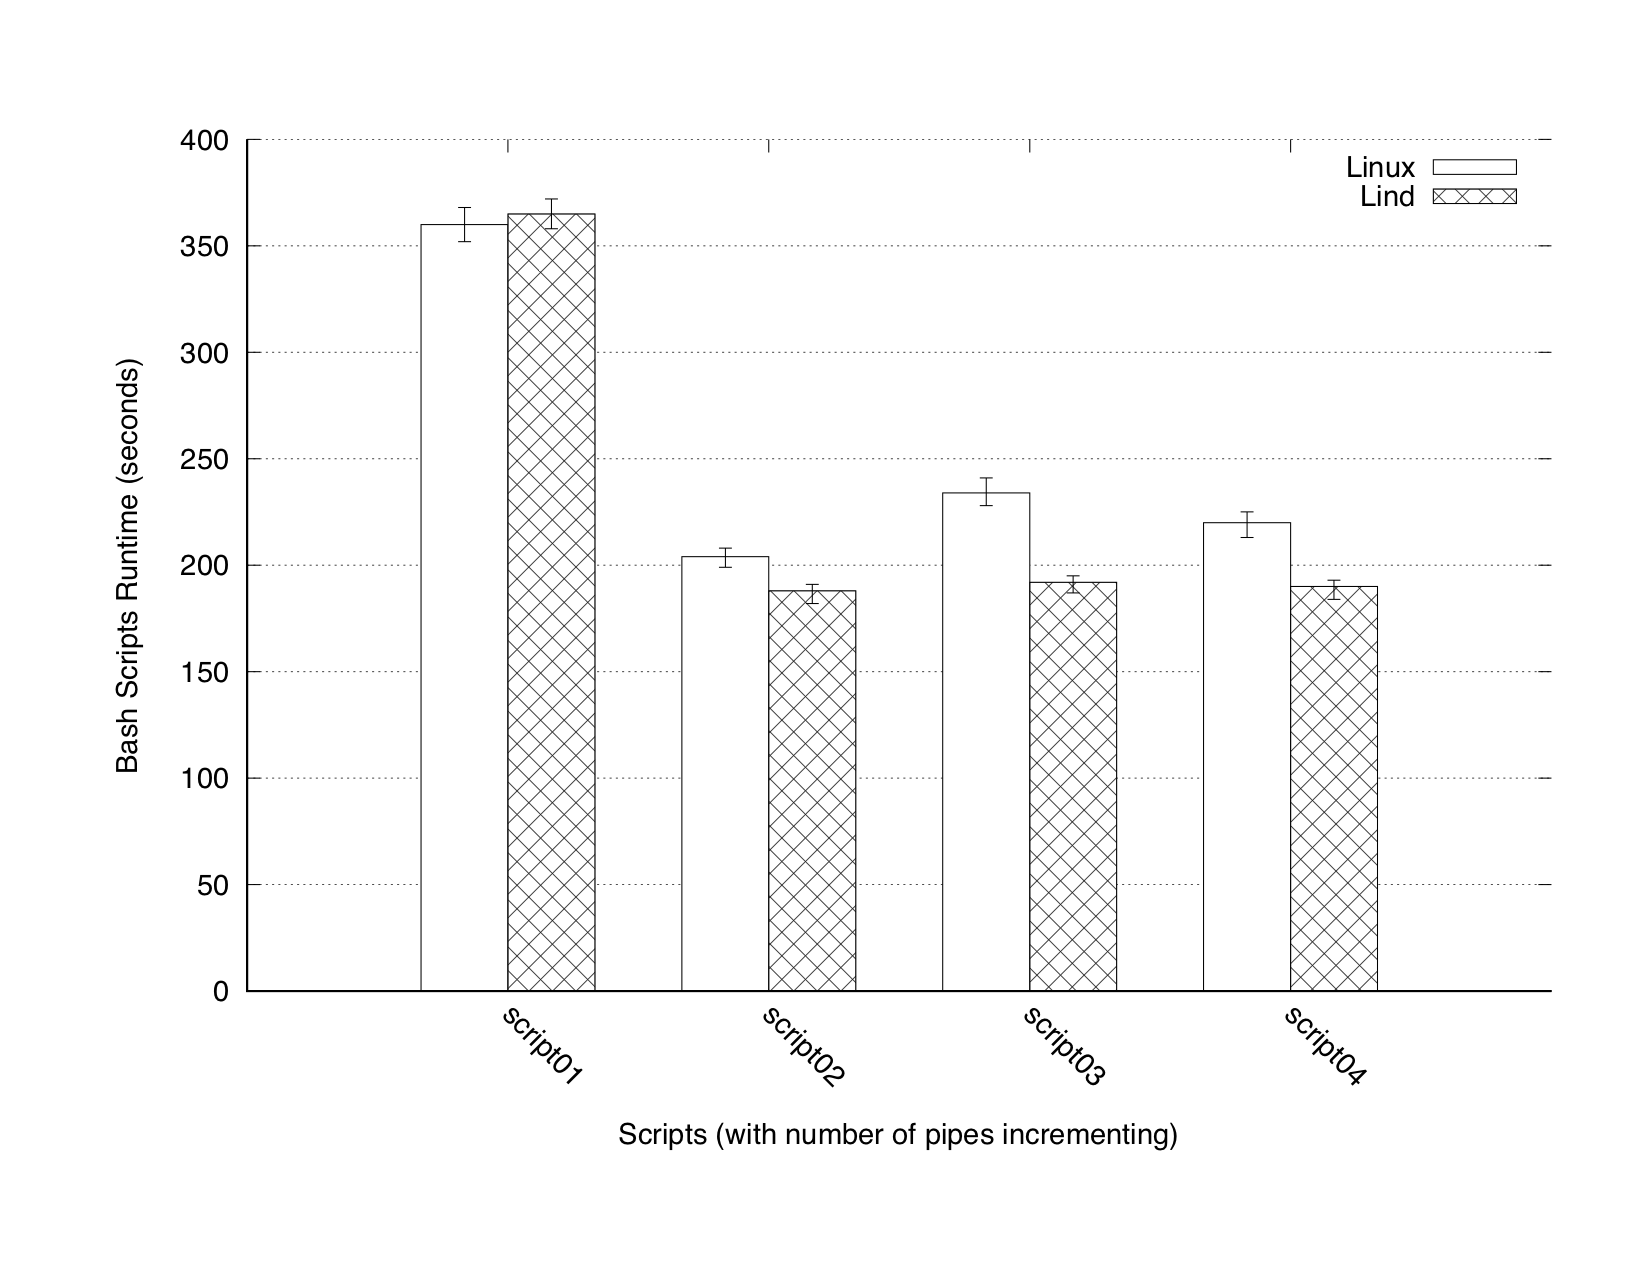
\includegraphics[width=1.0\columnwidth]{diagram/results02.png}
\caption{\small Real-World Workload 2.}
\label{fig:results02}
\end{figure}
\section{Discussion}
\label{sec:discussion}

\section{Conclusion}
\label{sec:conclusion}


\bibliographystyle{abbrvnat}
\bibliography{biblio}

\end{document}
